%=================AVANCES Y PRUEBAS=================
% SENSORES DE PULSO

\section{Pruebas SIT}

Una vez realizadas las pruebas unitarias de los diferentes módulos con los que cuenta In-Help y estas siendo exitosas, se procedió a realizar la integración de los módulos, posteriormente, se realizaron pruebas de los flujos críticos de operación In-Help, esto con la finalidad de asegurar el correcto funcionamiento. Para poder explicar el flujo completo que debe seguir un usuario, lo representamos con tareas generales, mismas que se observan en la figura \ref{fig:FNSIT}.

Para comprobar el funcionamiento de la aplicación se realizaron pruebas de integración con los diferentes módulos de la aplicación, esto hasta llegar al objetivo, notificar a contactos de emergencia, ya sea de forma manual o automática.\\


\begin{figure}[htbp!]
	\centering
	\fbox{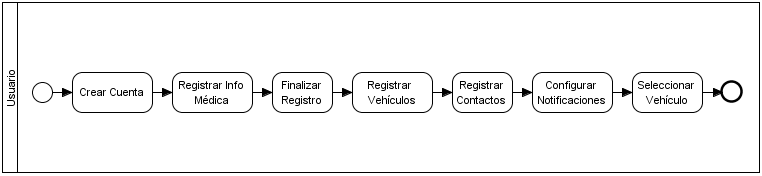
\includegraphics[width=1.1\textwidth]{AvancesPruebas/imagenes/Flujo_Notificacion}}
	\caption{Flujo SIT Notificación Automáticas/Manuales}
	\label{fig:FNSIT}
\end{figure}

\subsection{SIT Notificaciones Automáticas}

Tomando como referencia la figura \ref{fig:Disparadores}, se generó un escenario haciendo uso de los valores que genera el giroscopio para poder así generar una alerta automática. Para comprobar el funcionamiento se presentan las siguientes figuras:
\begin{itemize}
	\item En la figura \ref{fig:LogGX} se muestra el valor que detecto el Giroscopio del smartphone, mismo que esta fuera del rango establecido, por lo cual se esperaría la generación de una notificación automática.
	\item En la figura \ref{fig:GxNotifica} se muestra el mensaje de notificación automática para el usuario, que si no cancela generará un registro y enviará la notificación.
	\item En la figura \ref{fig:GxAPI} se muestra la información que se guarda en la BD después de que el usuario no cancelo la notificación automática.
	\item En la figura \ref{fig:GxVisualiza} se puede observar la notificación que se generó para el usuario.
	\item En la figura \ref{fig:GxMSN} se puede visualizar la información que se envió, con base en las configuraciones.
\end{itemize}

\begin{figure}[htbp!]
	\centering
	\fbox{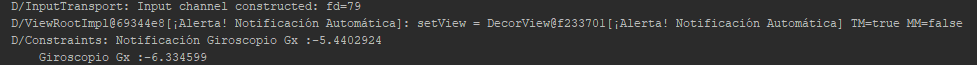
\includegraphics[width=1.0\textwidth]{AvancesPruebas/imagenes/GxLog}}
	\caption{Log Giroscopio Android}
	\label{fig:LogGX}
\end{figure}

\begin{figure}[htbp!]
	\centering
	\fbox{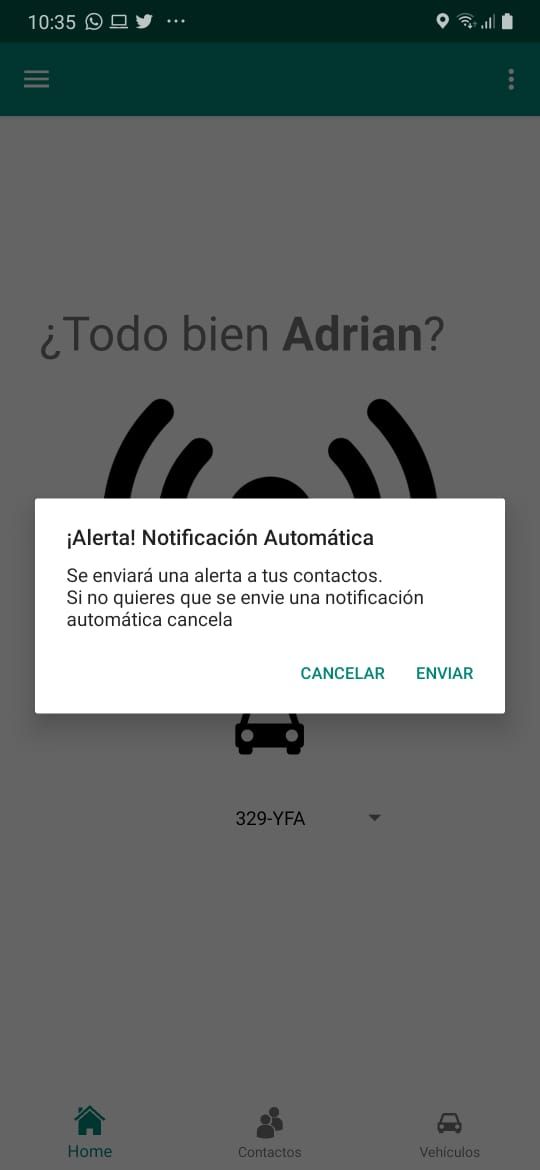
\includegraphics[width=.3\textwidth]{AvancesPruebas/imagenes/GxNotifica}}
	\caption{Alerta Notificación Automática}
	\label{fig:GxNotifica}
\end{figure}

\begin{figure}[htbp!]
	\centering
	\fbox{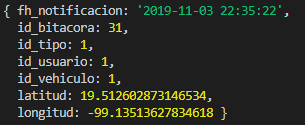
\includegraphics[width=.5\textwidth]{AvancesPruebas/imagenes/GxAPI}}
	\caption{Datos de Notificación Automática}
	\label{fig:GxAPI}
\end{figure}

\begin{figure}[htbp!]
	\centering
	\fbox{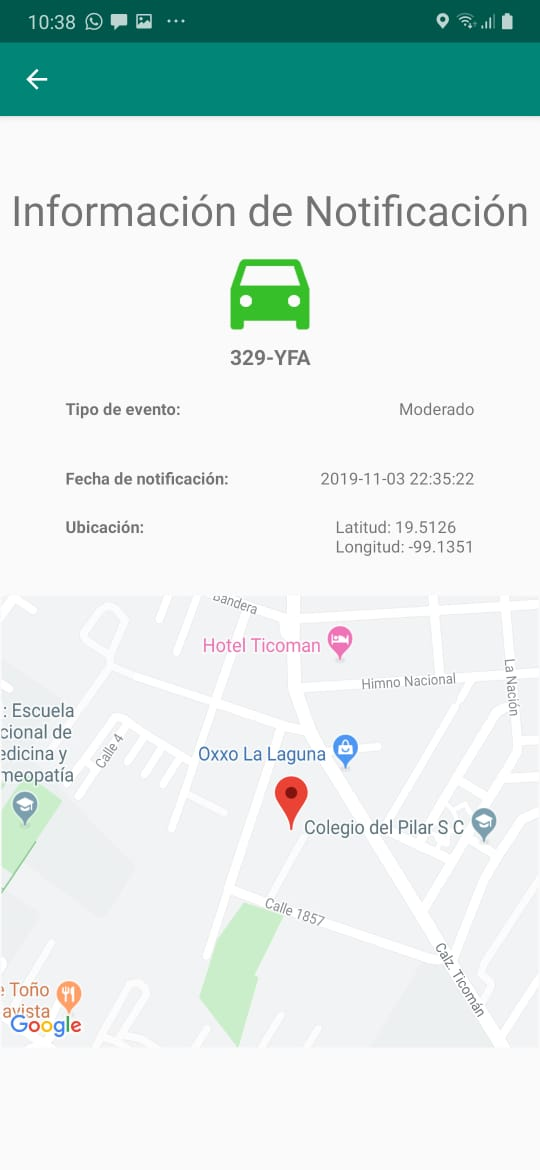
\includegraphics[width=.3\textwidth]{AvancesPruebas/imagenes/GxVisualiza}}
	\caption{Visualización de Notificación Automática}
	\label{fig:GxVisualiza}
\end{figure}

\begin{figure}[htbp!]
	\centering
	\fbox{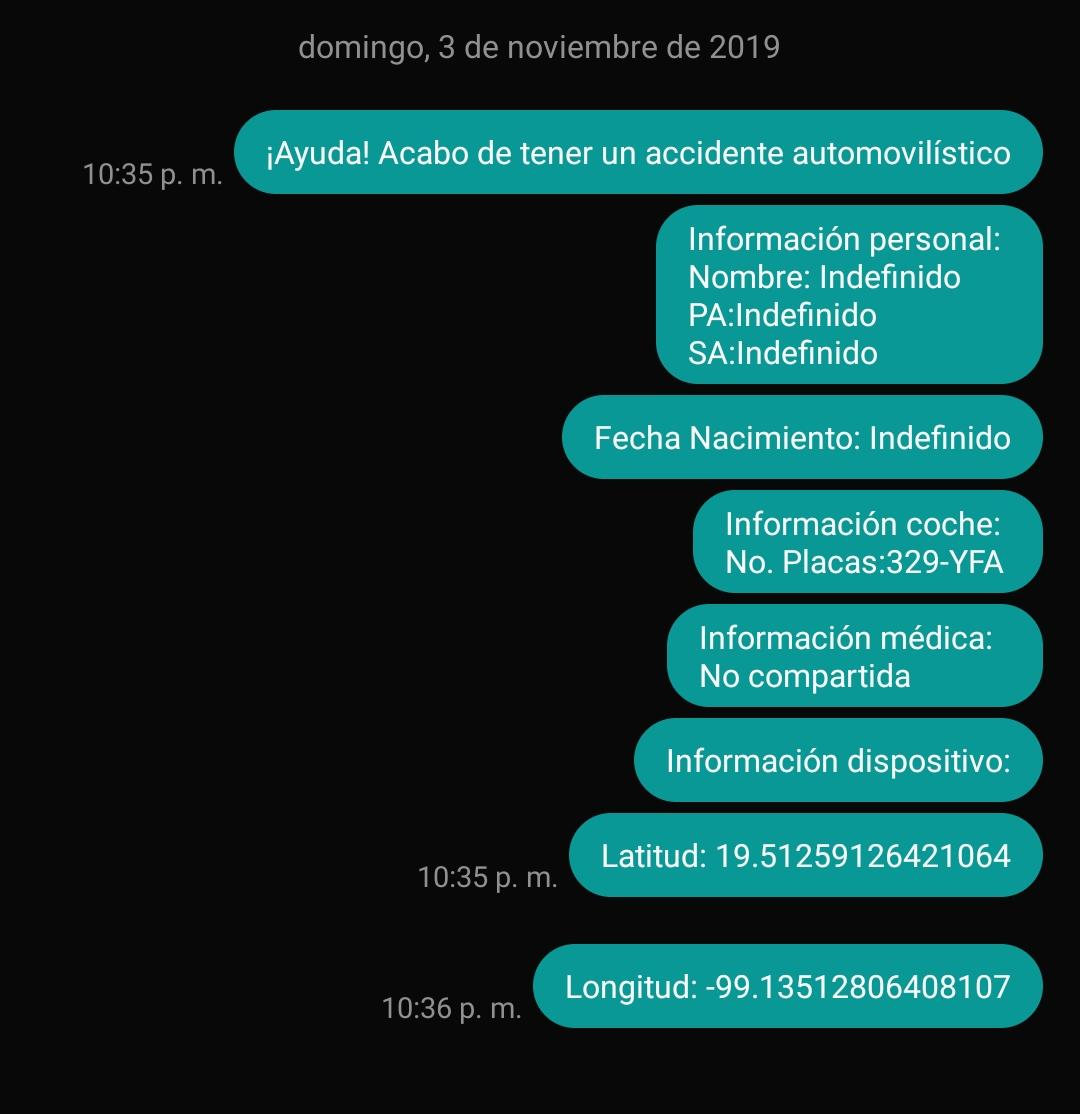
\includegraphics[width=.4\textwidth]{AvancesPruebas/imagenes/GxMSN}}
	\caption{Mensajes Enviado Notificación Automática}
	\label{fig:GxMSN}
\end{figure}



\subsection{SIT Notificaciones Manuales}

\begin{itemize}
	\item En la figura \ref{fig:GxNotifica} se muestra el mensaje de notificación manual para el usuario, y basta presionar ''ENVIAR" para que la alerta se envíe.
	\item En la figura \ref{fig:GxAPI} se muestra la información que se guarda en la BD después de que el usuario presiono el botón ''ENVIAR".
	\item En la figura \ref{fig:GxVisualiza} se puede observar la notificación que se generó para el usuario.
	\item En la figura \ref{fig:GxMSN} se puede visualizar la información que se envió, con base en las configuraciones.
\end{itemize}


\begin{figure}[htbp!]
	\centering
	\fbox{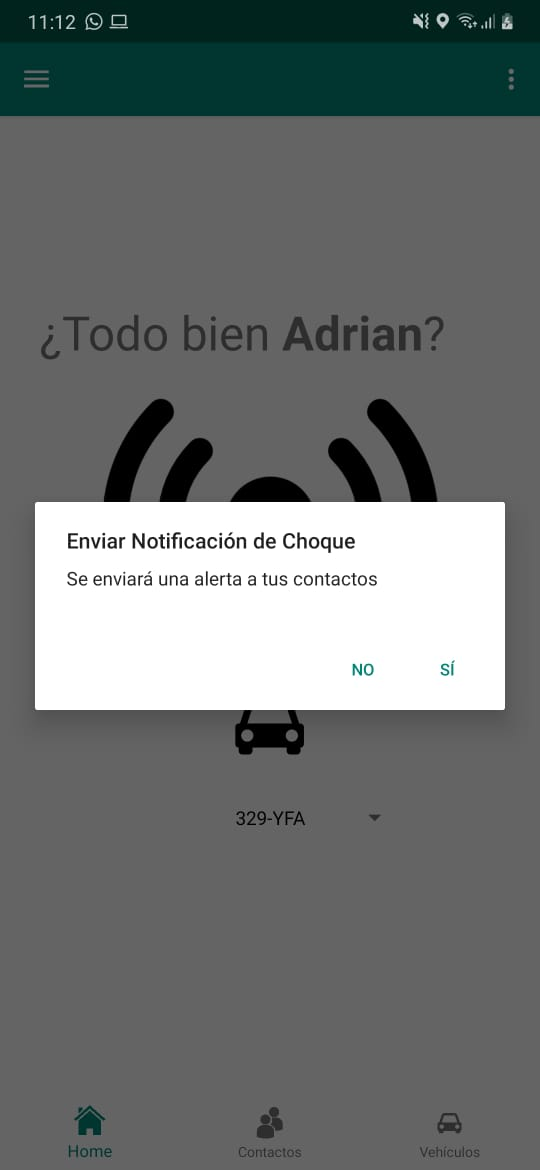
\includegraphics[width=.3\textwidth]{AvancesPruebas/imagenes/ManNotifica}}
	\caption{Alerta Notificación Manual}
	\label{fig:ManNotifica}
\end{figure}

\begin{figure}[htbp!]
	\centering
	\fbox{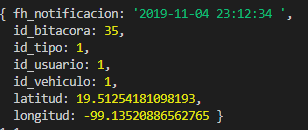
\includegraphics[width=.5\textwidth]{AvancesPruebas/imagenes/ManAPI}}
	\caption{Datos de Notificación Manual}
	\label{fig:ManAPI}
\end{figure}

\begin{figure}[htbp!]
	\centering
	\fbox{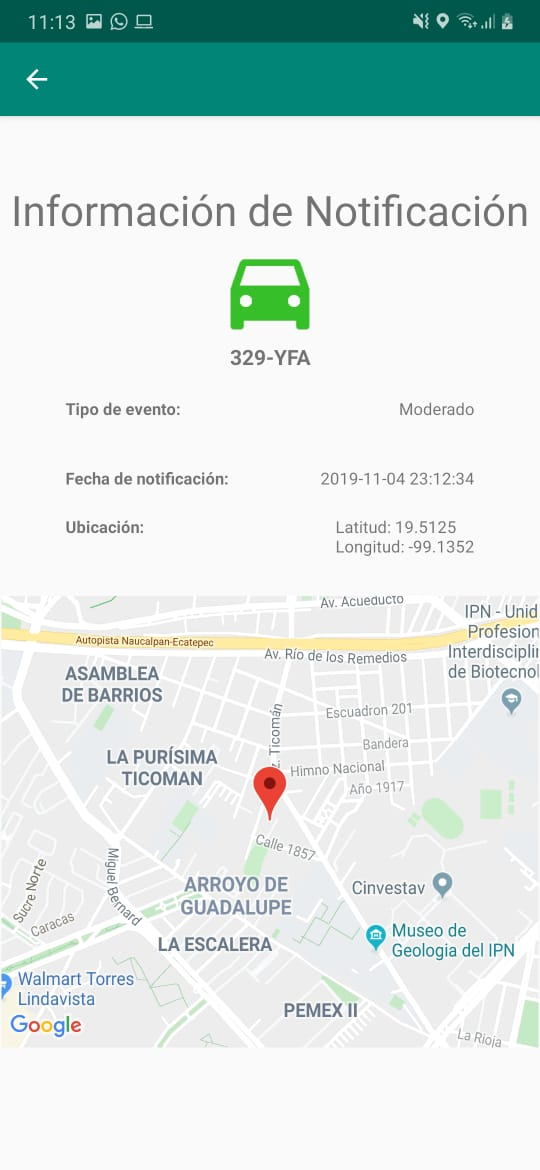
\includegraphics[width=.3\textwidth]{AvancesPruebas/imagenes/ManVisualiza}}
	\caption{Visualización de Notificación Manual}
	\label{fig:ManVisualiza}
\end{figure}

\begin{figure}[htbp!]
	\centering
	\fbox{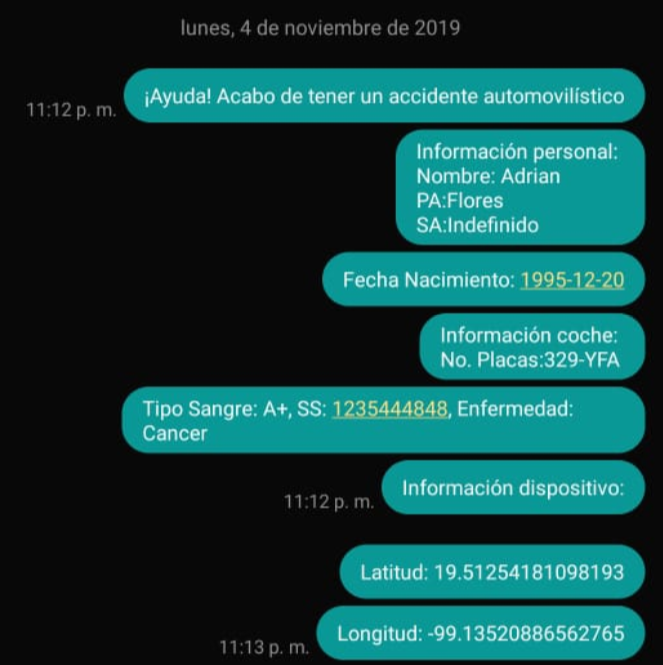
\includegraphics[width=.4\textwidth]{AvancesPruebas/imagenes/ManMSN}}
	\caption{Mensajes Enviado Notificación Manual}
	\label{fig:ManMSN}
\end{figure}



 